\documentclass{deliverablereport}

\usepackage[style=alphabetic,backend=bibtex]{biblatex}
\usepackage{todonotes}
\usepackage{pdfpages}
\addbibresource{report.bib}
\addbibresource{../../lib/publications.bib}

\usepackage{xparse}
\usepackage{xspace}
\usepackage{etoolbox}
\usepackage{caption}

\usepackage{graphicx}

\deliverable{dissem}{ibook3c}
\duedate{31/07/2019 (M47)}
\deliverydate{31/07/2019}
\author{Hans Fangohr, Thomas Kluyver, Marijan Beg, Min
Ragan-Kelley, Vidar Fauske, Marcin Kostur, Jerzy \L{}uczka
 }

\newcommand{\sagenb}{SageNB\xspace}
\begin{document}
\maketitle
\githubissuedescription
\newpage
\tableofcontents
\newpage


\section{Introduction}

Interactive web pages have always been an attractive tool in
education. In \longdelivref{dissem}{ibook1} we have presented example of
interactive books, which can contain not only animations or widgets
but also due to \texttt{@interact} decorator and ``sagecell``
technology, can be modified and extented while reading.

On the other hand a well estabilished tool for experimentation is a
notebook interface. It posseses also a capabilities requite for rich
text authoring. Here, we deliver two interactive books: Problems in
Physics\footnote{\url{https://github.com/marcinofulus/Mechanics_with_SageMath}\\%
\url{https://github.com/marcinofulus/Dynamical_Systems}\\%
\url{https://github.com/marcinofulus/Transport_Processes}}%
%
and ``Introduction to Python Computational Science and
Engineering``\footnote{\url{https://github.com/fangohr/introduction-to-python-for-computational-science-and-engineering}}. We have used \Jupyter notebook as a common platform for
both prototyping the code and experimentaion as well as authoring the
manuscipt. We will also present two workflows and ``cookie-cutter``
repository which allows easy start for anyone interested.


The main conclusion of this work is that the \Jupyter notebook-only
solution provides a way to write a high-quality book containing
scientific computations. Due to \ODK effords we managed not only to
lower barriers for including computations in science education but
also significantly improve maintanability of such interactive
materials by proper use of automated validation.

We have also demonstrated that the approach in
\delivref{dissem}{ibook1} and notebook based workflow (here) are
complementary and can be used dependent on the situation. Notebook
based workflow is better for computer science based topics or
problem-oriented books. It clearly has a lower barrier for Authors,
collaboration is also easier, especially for people who are not
excellent in ICT. While working with various faculty members at
University of Silesia, it was possible to have some of them to do
pull-request on github server, but some where just editing independent
notebook which was later manually copied and merged with repository be
other person.


\section{Reducing barriers for learners and teachers using interactive textbooks}



\subsection{Learners perspective}

The \Jupyter notebook as a virtual research environment holds great
potential for the creation and use of interactive documents. In this
context, we investigate and prototype the use of such interactive
notebooks in the context of education at the university level.

There is a long history in academia to provide textbooks either as
the main point of reference for a given lecture course, or as an
additional "background reading" to provide more details which cannot
be covered by blackboard- or slide-centered lectures, typically due to
the lack of time available.
%
While providing potentially a wealth of information, such textbooks
are static, and require unusual skill to be exclusively learned
from. Instead, it is a common model to ask students to carry out
practical problem-solving exercises: this enforces engagement with the
material and supports deep learning of the subject.

For computational problems, there is often significant effort required
to set up an environment of software (such as Python with required
libraries or a symbolic mathematics package) and then to set up a
problem environment that allows the study of the topic under
investigation. For example, to solve a differential equation
numerically, the problem environment includes setting up functions
describing the ODE, boundary conditions, and a grid on which the
numerical solution should be obtained. Once this point is reached, the
student can start to explore -- for example -- the properties of a
numerical method being used to solve differential equations.

The \emph{interactive textbooks} developed here allow to improve the
learning experience by significantly reducing this barrier: both
setting up the software environment and setting up the problem
environment are reduced to the task of opening the interactive
document in a browser for which the teacher provides the URL. A short
wait while the virtual environment is created on the fly (using the
Binder service) and navigating to the point of interest in the
textbook. Immediately, it is possible for the learner, to
interactively explore the topic of learning within a prepared learning
and software environment.

Students can access the notebooks and inspect all the computational
steps that have created the results shown in the textbook. Assuming
they have the relevant software installed, they can execute them on
their own machine, modify, explore, understand, and extend the
examples. As all computational steps are included in the notebooks,
there is no guessing about assumptions, no code being executed before
an example is introduced, or no reconstructions of sections labeled
``the required transformation of X is left as an exercise to the
reader'' required: all steps are contained in the notebooks. This
reduces the barrier towards learning.



\subsection{Teachers perspective}

The ease of authoring manuscripts is a key to wide application of any
good practice described in this report. Generally speaking, academic
teachers lecturing on computer science tend to be fluent in all kinds
of computer technology and happily adopt new ones. However, as topics
get further and further from computer science as in theoretical
mechanics or dynamical systems technology, technology literacy becomes
a barrier. It can often happen that such subjects are not integrated
with computer technologies during teaching at all.


University of Silesia has engaged into the introduction of \SageMath
into science education ever since 2011\footnote{\SageMath, or \Sage
  for short, is an open source, community developed, Python based
  general purpose computational system for (pure) mathematics}.
Initially, the \sagenb notebook server was
used as to serve both as computational resources and as course
material distribution center. Despite its clear limitations, it has
been widely adopted and was used in many courses. In its peak load it
was serving on average one computation per second to 2000 registered
students. The number of created by students notebooks exceeded
20000. Many academic teachers appreciated the fact that our 'cloud'
installation required merely to login in order to start working. This
feature of the central \sagenb turned out to be so important, it had to
be preserved when developing a new solution

Eventually \sagenb showed its limits due to its small developers
community, and we seek for a sustainable and more flexible alternative
which would allow for use not only in physics and mathematics but also
for e.g. computer science or biology. The \Jupyter ecosystem, with
versatile tools and use cases, had become an obvious candidate. Still,
there were many questions to be resolved around the migration path
(e.g. how to convert old materials) and the optimal use of those tools
in practice.  \ODK project provided solutions to most of those
questions. First, in \longdelivref{UI}{ipython-kernel-sage} the
\SageMath kernel for \Jupyter notebook was finished enabling using the
same formath for both \Sage as well as \Python based
documents. Additionally, in \delivref{UI}{ipython-kernel-sage} the
conversion tool was provided, which enabled to simplify the migration
from \sagenb. 

In the following, we detail the work on the interactive textbooks:
``Computational Science and Engineering'' (Sec.~\ref{sec:computational-science-and-engineering})
and ``Problems in Physics with \SageMath'' (Sec.~\ref{seq:problems-in-physics}).
Then we reflect on our experience with Jupyter based interactive
textbooks, both from the learner and author perspectives (Sec.~\ref{sec:auth-using-inter}).

\subsection{Cats perspective}

\includegraphics[width=10cm]{cat.jpg}



% \todo[inline]{Viviane/Nicolas, please update as required.}

\section{Interactive text book on Computational Science and Engineering}
\label{sec:computational-science-and-engineering}

\subsection{Context and overview}


The application of mathematics in science and engineering is the topic
of the textbook "Introduction to Python Computational Science and
Engineering".
%
The target audience is scientists outside computer science. It is
thus important to teach some programming basics before using those to
conduct computational and data science tasks.

The work is based on a textbook that was available as a PDF file (and
generated from a \LaTeX{} file). In this deliverable, we have reviewed
the textbook and updated it from Python 2 to Python 3, added various
sections and a chapter on Pandas, but most importantly translated the
\LaTeX{} sources into \Jupyter notebooks. Furthermore, we used and
evaluated tools such as \texttt{bookbook} and \texttt{nbconvert} to
automatically convert the textbook in alternative formats.

The new PDF is created from the \Jupyter notebooks by auto-generating
\LaTeX{} sources compiling them to create a high quality PDF file. A
\LaTeX{} file with custom style settings can be given as a template to
the \texttt{bookbook} package. The different chapters (each being one
notebook) are merged automatically, and get a joint table of contents.

From the same \Jupyter notebook sources, a set of HTML files can be
created to allow more convenient online reading of the material. These
HTML files are organized into one HTML file per chapter (each being
created from one notebook), and an additional index file providing
links to all chapters.

The (automatic) translation of the \Jupyter notebook-based textbook
into PDF is important to provide (at least) the same level of
publication quality outputs that can be expected from the more
traditional \LaTeX{} based manuscript. The conversion to HTML is an
added bonus, and offers a way of reading the document that is more
appropriate for commonly used devices such as laptops, tablets, and
smart phones.

%\TODO{Is thebelab enabled on the HTML version?}

\subsection{Availability}

The complete book is open source and available from\newline
{\tiny\url{https://github.com/fangohr/introduction-to-python-for-computational-science-and-engineering}}\linebreak
under a Creative Commons license (Attribution-NonCommercial 4.0
International (CC BY-NC 4.0)).

A Zenodo entry has been created (\url{https://doi.org/10.5281/zenodo.1411868}).

\subsection{Uptake and feedback}

The textbook is used regularly at the University of Southampton to
teach all engineering students about computational science in their
first year of studies (typical numbers of students per year between
300 and 500). The physics department has also started to adapt these
materials. Due to Prof. Fangohr's move to European XFEL and the
University of Hamburg, the textbook is also in use in optional
courses at the Physics department to provide an introduction to
computational science.

We know from instructors at other institutions that they are using the
textbook in their teaching, including Aalborg University (Denmark),
University of Hamburg (Germany),
Haverford College (Pennsylvania, US), Tulane University, New Orleans
(US), GeorgiaTech, Georgia (US), University of California, Santa Cruz,
California (US), University of South California, Los Angeles
(US), Federal University of Paraiba, Paraiba (Brasil), University of
Virgin Islands, Virgin Islands (US). Some of these courses are
in the area of computational science and data science, but most
are outside computer science and addressing engineers, biologists,
meterologists, chemists etc.

We have also heard from individual students that participate in other
courses at universities or courses from Coursera and who have enjoyed
the textbook as a freely available complement, providing static and
interactive learning material.

A translation into Portuguese is available, including the interactive
version on Binder.\footnote{https://github.com/gcpeixoto/lecture-ipynb/blob/master/README.md}
\pagebreak



\section{Interactive text books: Problems in Physics with \SageMath}
\label{seq:problems-in-physics}


\subsection{Context and overview}

Problems in Physics with \SageMath is a set of lecture notes collected for
over one decade during teaching activities at University of
Silesia. Topics range from classical mechanics to dynamical systems
and transport processes. Those materials have been used for teaching
in following courses: Theoretical Mechanics, Introduction to fluid
dynamics, Programming massively parallel processors in CUDA,
Mathematical Methods in Biophysics.


At the University of Silesia (Institute of Physics), the content of
the material in the e-books has been exploited for many years as parts
of lectures and exercises for two groups of students: the second year
of study of biophysics (Mathematical Methods of Biophysics) and the
fourth and fifth year of physics study (seminars and monograph
lectures). In summary, about 100 students participated in the above
courses. From our experience it follows that in particular it has been
useful for students of biophysics who are less fluent in calculations
and transformations of mathematical expressions. The possibility of
graphical presentation allows them to acquire intuition and better
understanding of properties and behavior of some processes and
phenomena.

\subsection{Availability}

The complete book consists of three parts and are  open source and available from:\newline
{\url{https://github.com/marcinofulus/Mechanics_with_SageMath}\linebreak
{\url{https://github.com/marcinofulus/Dynamical_Systems}\linebreak
{\url{https://github.com/marcinofulus/Transport_Processes}\linebreak
under a Creative Commons license (Attribution-NonCommercial 4.0
International (CC BY-NC 4.0)).

\subsection{Part I: Classical Mechanics with \SageMath}

This book contains set of problems solved with the help of computer
algebra. It consists of \Jupyter notebooks and uses  \SageMath kernel.

Problem solving problem in classical mechanics often require an hour
or more of paper and pencil algebra. It is mostly connected with
formulas which appear during change of coordinates in various
expressions and differentiation. Derivation of Euler-Lagrange
equations for double pendulum in polar coordinates can be a prominent
example, in which expressions easily take two lines of handwriting.
Although very informative, such derivations may first of all discourage
the student from further analyzing the system, and secondly, there is
a growing chance of making a mistake with the length of equations.

Instead of scaring students with lengthy formulas these tasks can be
quickly done with the help of Computer Algebra Systems
(CAS). Mechanics with SageMath consist of a set of notebooks in which
we solve classical problems in mechanics. Our approach differs from
the traditional one in:
\begin{enumerate}
\item It is insisted that all derivations are done automatically with
  help of CAS,
\item When equation of motion are obtained algebraically, we use
  numerical and algebraic method to analyze the system.
\item Wherever possible we create visually appealing pictures or
  animations which illustrate the key properties of the system.
\end{enumerate}

This approach requires the reader to take time to learn about the
computer algebra system and programming. However we believe that this
knowledge will give disproportionately larger benefits and will not
only make problem solving in mechanics a pleasure but prepare to solve
real life problems where analytically tractable formulas are not so
common.



\subsection{Part II: Dynamical Systems}

The interactive book "Dynamical Systems" has its source in teaching
students of Econophysics at the Faculty of Mathematics, Physics and
Chemistry (University of Silesia). Next, the content of this course
has been extended to students of theoretical physics and
biophysics. This course is very attractive for using Sage. Applying
Sage, it shows that analysis of some classes of dynamical systems (as
a set of differential equations) is much more simpler and it allows to
understand even complicated behavior of processes appearing in natural
sciences.  This course starts with motivation of using differential
equations for modeling of some processes in physics, biophysics and
econophysics. Fundamental information on a set of autonomous
differential equations is presented with minimal mathematical
apparatus. Very impressive are examples showing non-uniqueness of
their solutions. Elementary notions like phase space, phase curves and
vector fields associated with differential equations are introduced
and examples are shown by using Sage. The next section of the e-book
concerns attractors. Again, various classes of attractors can be
presented for differential equations by applying Sage. In classical
mechanics, conservative and dissipative systems play a crucial role in
understanding statistical physics, irreversible processes and chaotic
properties of deterministic systems. It is a subject of one of the
section. The final part of the book is devoted to a difficult notion
of deterministic chaos. As an example, we consider a classical
particle moving in a bistable potential and driven by a time periodic
force. In this part, Sage appears to be extremely useful in visual
demonstration and understanding of chaotic properties of relatively
simple dynamical systems. Without Sage it would be impossible to apply
any analytical and tractable methods to obtain desired information on
this system.


\subsection{Part III: Transport Processes}

The interactive book ``Transport Processes'' is based on two courses
taught in Institute of Physics at University of Silesia: Introduction
to fluid dynamics, Programming massively parallel processors in
CUDA. Those courses were intended for graduate students and PhD
students. In both courses we followed problem oriented
teaching. Student were given a \Jupyter notebook with introductory
information and the problem statement. After some time of individual
work solution were returned. In this cases grading was performed
manually, usually followed by discussion of problems and methods of
solution individually with a student.

\subsection{Outlook and future work}

A new academic year 2019/2020 starts with the new and big Faculty of
Natural Sciences and Technology. Therefore the e-books will be used
for wider audience of students, not only in physics but also in
material sciences and computer sciences. Our colleagues from other
Polish higher schools are also interested in using the presented
e-books.


\section{Authoring and using interactive textbooks}\label{sec:auth-using-inter}

\subsection{Tools and best practices for authoring Jupyter based
  interactive textbooks}\label{sec:good-pract-softw}

During the four years of this project we have experimented with many
different ways to effectively author and distribute material, and in
particular large structured documents such as textbooks.

In \longdelivref{dissem}{ibook1} we have explored the use of the
sphinx documentation system. This offers very high quality output to
html and pdf, strong cross-references support, and smooth integration
in the usual developer toolkit (editor, version control, testing,
...). We managed to implement in addition embedded sagecell for an
interactive html version. The major disadvantage is, however, a non
negligible barrier for many authors: they have to learn ``yet
another`` authoring tool and need to have some minimal fluency in ICT
to be able to perform edit-compile-view cycle.

In contrast, for this deliverable we explored authoring the books
directly as a collection of \Jupyter notebooks, bound together with
the \texttt{bookbook} tool to generate outputs in various formats. Our
authors found very convenient that the same environment could be used
all the way for prototyping exercises to authoring the manuscript
itself, and that the prerequisites were minimal. In this case the
superior flexibility of sphinx system was sacrificed for simplicity.

All technologies developed in this work-package can be transferred to
the European Open Science Cloud in fairly straightforward manner, as
the communication protocol is HTTPS, and all data is written in
structured machine-readable formats.

\bigskip

There are many ways to work with notebook-based source materials.  We
have used the technologies and processes described below to improve
the quality and maintainability of the open source textbook. We
distringuish two cases, which differ in very first decision - if one
wants to keep output of the notebooks in version control or not.

\subsubsection{Workflow I - notebooks with output}

In this case we assume that notebooks are committed to a version
control system (typically git) with output-cells. It gives the author
the option of later using this output for automated testing. The
live-example of this scenario is the book ``Introduction to Python
Computational Science and Engineering''.

In order to make most out of this worlflow we have used the following
technologies and processes to improve the quality and maintainability
of the open source textbook.
\begin{itemize}
\item The sources are available and publicly readable on
  Github\footnote{https://github.com/fangohr/introduction-to-python-for-computational-science-and-engineering}
\item Changes in the files are tracked through commits in Git.
\item Together with the executable textbooks, we have defined
  \emph{automatic tests} that can re-execute all material in the
  notebook to check that the newly calculated outputs match
  up to trivial differences, with the recorded outputs.
  This uses the \nbval tool -- developed as part of
  OpenDreamKit\footnote{ See \longdelivref{UI}{jupyter-test} }.

  If deviations or even exceptions arise, then the displayed example
  output is not generated from the computational input, and thus the
  chapter is outdated (or simply wrong). For conventional
  (non-interactive) textbooks, such gradually becoming outdated is
  hard to recognize, and typically updated with the next edition a
  few years later.

  In the context of this textbook, there are two common sources for
  deviations reported by \nbval:
  \begin{enumerate}
  \item Changes in the chapter have had (unexpected) side effects
    later in the chapter, combined with a failure to re-execute the
    whole chapter manually to check for such deviations after the
    changes were introduced.
  \item Changes in libraries we depend on: for example, the change to
    Matplotlib version 3 has introduced new behaviour of Matplotlib,
    which resulted in different outputs.
  \end{enumerate}

\item These automatic tests are executed whenever changes are
  committed to the repository, or when a branch is requested to be
  merged into the master branch. We use Travis CI for this, which
  provides this service free of charge for open repositories\footnote{\scriptsize
  \url{https://travis-ci.org/fangohr/introduction-to-python-for-computational-science-and-engineering}}

  This makes it feasible to consider community contributions to the
  textbook: at least the internal consistency of input and output for
  any contribution is checked automatically, even before the author
  team starts reviewing the proposed changes or additions.

\item We use (Docker) containers on the Travis CI testing system to
  host the software environment within which the notebooks are
  executed and converted to generate the PDF and HTML version, and we
  also use this container environment to compare input and outputs
  (using \nbval, see above).

  Using containers here has the following advantages:
  \begin{enumerate}
  \item Through the \texttt{Dockerfile} (and the \texttt{.travis.yml}
    file), the building of the container is fully defined: users who
    want to also convert the notebooks to HTML or PDF, or re-recreate
    what is done on the continuous integration system, can either
    create the same container, or follow the installation on a virtual
    machine or bare metal machine. In any case, having these
    configurations available is more explicit than using the default
    Linux and configuration that Travis CI provides.

  \item If a problem arises in the continuous integration, we can
    replicate the same environment locally (in a Docker container on
    our own workstation/laptop) and fix it there: this is more
    effective than having to commit to the repository and to wait for
    Travis CI to re-execute the tests to check if the problem has
    disappeared.

  \end{enumerate}

%\newpage\printbibliography
\end{itemize}


\subsubsection{Workflow II - notebooks without output}

We have applied this workflow to Problems in Physics books, testing it
against \SageMath and \Python. In principle it is language agnostic
and will work with any \Jupyter kernel. Key concepts of this scenario
are following:

\begin{enumerate}
\item As above, the source notebooks are available in a public
  repository, e.g. on GitHub, and changes in the files are tracked
  by version control, e.g. with Git.
\item The notebooks are stored, however, without outputs.
\item a ``Makefile`` is used to automatize the processes: building of
  the pdf and html versions, etc.
\item \nbconvert is used to automatically execute and clean notebooks
  and to produce the pdf and html versions.
\item The conversion to html can produce interactive figures (such as
  \texttt{@interact}). Alternatively, it can produce static figures in
  `pdf`. This is configured by the environment variable
  \texttt{os.environ['PDF']}.
\item Regression tests can be embedded in the notebook, as input cells
  marked with an ``nbtest`` tag. Such cells are removed during the pdf
  or html conversion.
\item A \texttt{Dockerfile} is provided which allows to run a given
  repo on mybinder service.
\end{enumerate}

Clearly, not all parts are mandatory. For example one can skip
regression tests or interactive figures, at least at the initial phase
of authoring.

We produced a template repository \footnote{\scriptsize
  \url{https://github.com/OpenDreamKit/authoring_cookie_cutter}} which
authors can use to initiate their own textbook project. It can be
easily adapted to one's own needs. It contains a Binder link, which
enables anyone to try the notebooks interactively.

Here is the workflow in practice:
\begin{enumerate}
\item Setup a directory and software environment ( e.g. starting from
  ``authoring\_cookie\_cutter``)
\item Create/edit or modify notebooks
\item Run ``make pdf`` and/or ``make html``. As a side effect, errors
  are cleared.
\item Check the outcome and commit.
\end{enumerate}

Interestingly, since the notebooks do not contain output, building the
pdf or the html will re-execute the whole book, stopping at any error.
Hence this also serves as basic validation test, assuring that a
notebook will run from the top to bottom. This helps revealing side
effects of execution of cells accidently out of order.

The execution of the whole book can be computationally intensive; to
mitigate this, one can utilize the builtin multiprocessing
capabilities of \texttt{make}; for example, on a 4-cores system one
may use: \texttt{make html -j4} to run each individual notebook on a
different CPU core.

\subsection{Integration into MyBinder}



Using the cloud hosted \texttt{Binder} service
(\url{http://mybinder.org}), learners can open the book in an
temporary \emph{Virtual Research Environment (VRE)} that has been
created on demand just for them. While providing all the advantages
outlined above, in this setup \emph{no software installation is
  required}.

In more detail in the case of ``Introduction to Python Computational
Science and Engineering'':




The following textbooks are available through MyBinder service: on the
github webpage of the books link to the MyBinder service is provided.

\begin{itemize}
\item ``Introduction to Python for Computational Science and Engineering''\footnote{\scriptsize\url{https://github.com/fangohr/introduction-to-python-for-computational-science-and-engineering/blob/master/Readme.md}}
The textbook can come with a specification of the software it requires
(for example through a Python \texttt{requirements.txt} file). For the
textbook at hand that specification is straightforward: indeed it
requires no software beyond the standard scientific Python stack
(numpy, scipy, matplotlib, pandas, \Jupyter, ...) which is included in
the default Anaconda Python distribution.

The textbooks and specification can be referenced by a URL. When a
student accesses this URL with his browser, the \texttt{Binder}
constructs on demand a Docker image including a copy of the notebooks
and the required software, and provisions a temporary Docker container
(lightweight virtual machine) running a \Jupyter notebook server. The
student can browse through the textbook, and execute chapter notebooks
as they like to achieve better


\item ``Mechanics with \SageMath''\footnote{\scriptsize\url{https://github.com/marcinofulus/Mechanics_with_SageMath/blob/master/README.md}}

In this case we use \texttt{Binder} with prebuild Docker image
\texttt{sagemath/sagemath:latest} which contains recent \SageMath
package. Similarily to previous case, all of interactive features can
be explored in notebooks opened in mybinder and \emph{no software
  installation is required}.


\end{itemize}

%% By clicking on it, the user is served a computational environment in
%% the cloud in which the textbook can be read, engaged with, and
%% interactively executed.

%% Additional links are provided to launch the notebooks in a JupyterLab
%% (rather than the classic \Jupyter Notebook) environment.

At the moment, this service is supported by funds from the \Jupyter
Project, but given ongoing development for the Binder project, and
interest from the European Open Science Cloud and various universities
and research facilities, it is likely that other MyBinder services
appear which can be used for such interactive document hosting in the
future. Of course there is a question over how this is financed -- one
possibility would be to finance this from overheads; comparable to
library costs and access to the Internet that are already accepted as
overheads in research and education.

Technically, we have specified our software requirements through a
\texttt{requirements.txt} file in the root of the repository. This is
the preferred way for Binder to read the specification, and also good
because we can express software requirements for execution of the
notebooks (which are relevant to learners) in this human readable
file.

When we build the container for the continuous integration (see
Sec.~\ref{sec:good-pract-softw}), we use a \texttt{Dockerfile} in a
subdirectory \texttt{docker/} (so that Binder does not see this file
as it would override the requirements provided in
\texttt{requirements.txt}), and when building the Docker image, we
pip-install all dependencies listed in the \texttt{requirements.txt}
file. We thus eliminate duplication of requirements completely.



\pagebreak
\appendix
\section{Appendix 1: Table of contents of the interactive book}\label{sec:appendix-1}

On the following 5 pages, we show the table of contents of the
interactive book \emph{Introduction to Python for Computational
  Science and Engineering}.
%
The full materials are available at
\newline
\url{https://github.com/fangohr/introduction-to-python-for-computational-science-and-engineering}

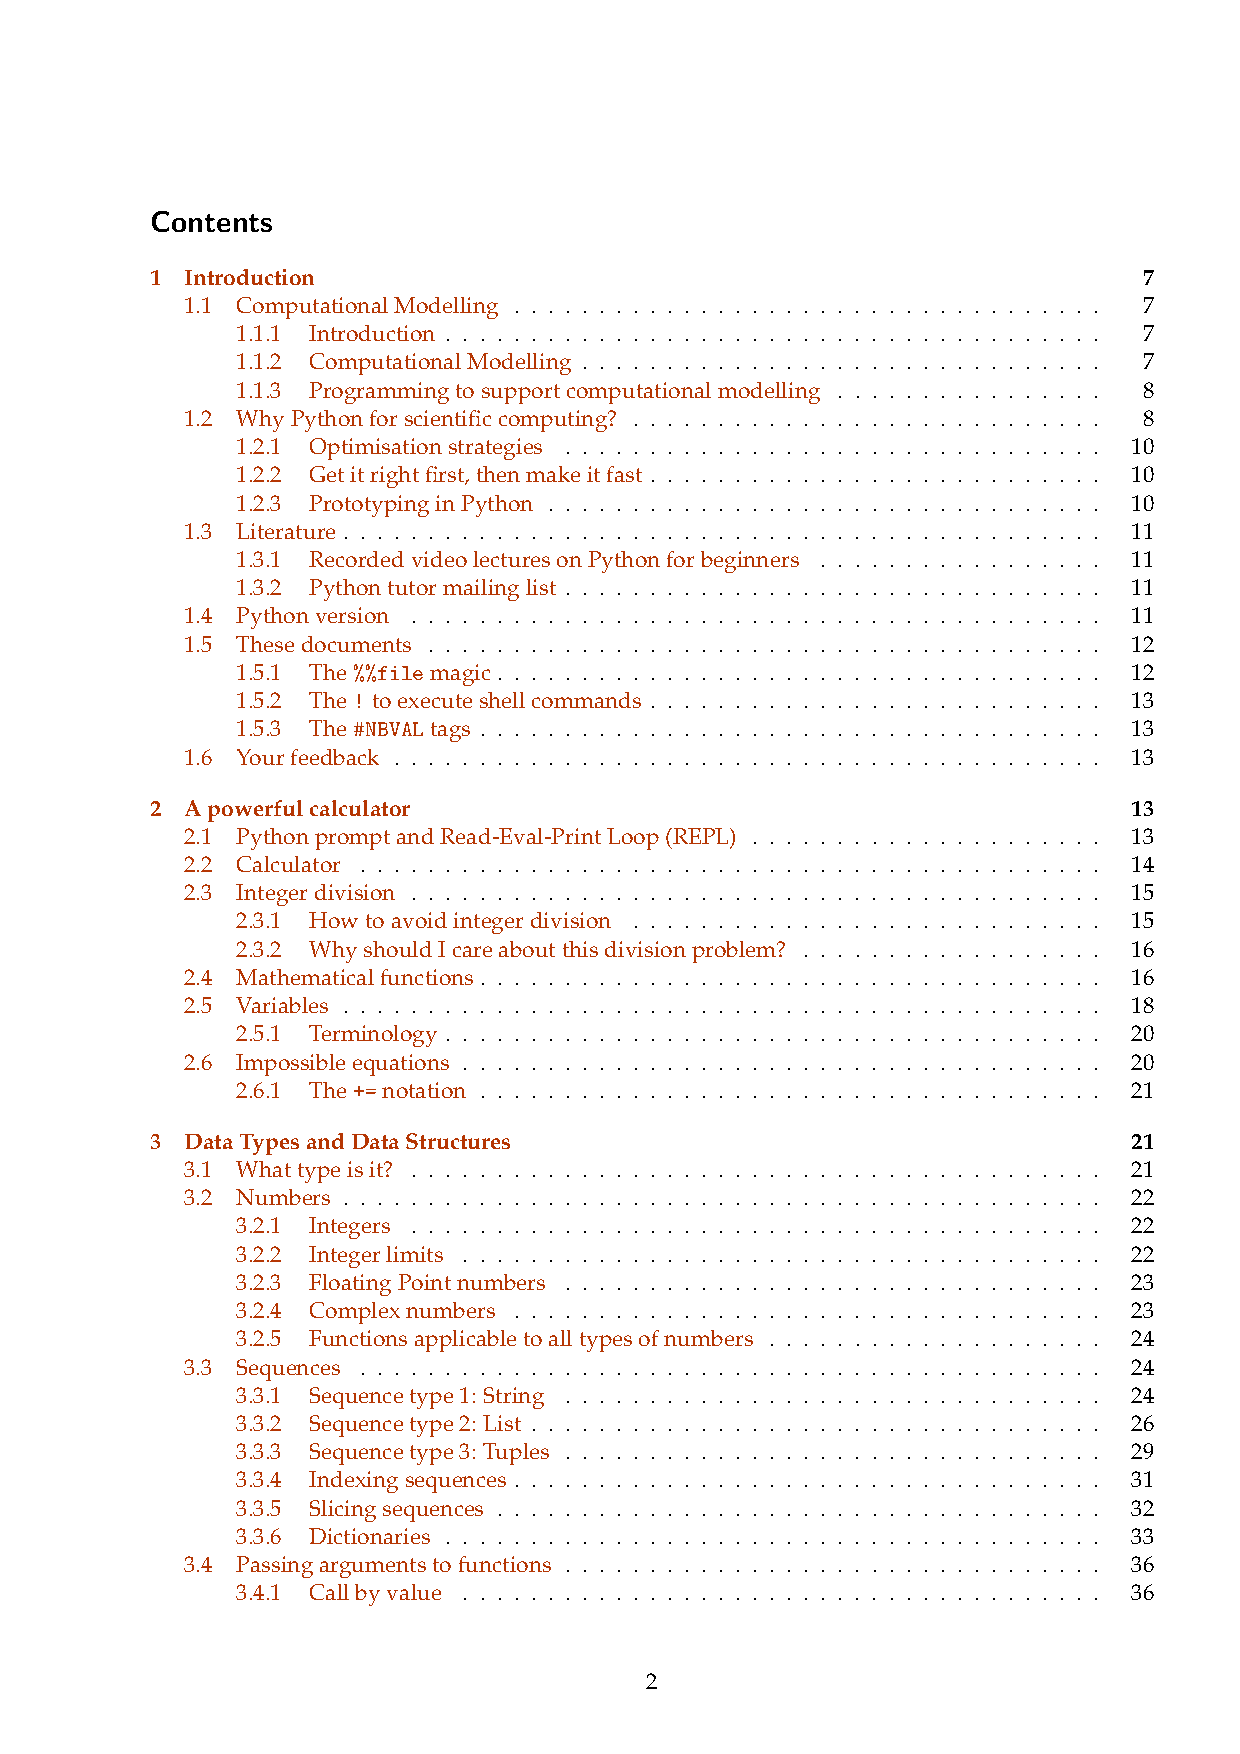
\includepdf[pages={1-5}]{computational-science-table-of-contents.pdf}



\section{Appendix 2: Table of contents of the interactive book}\label{sec:appendix-1}

On the following 5 pages, we show the table of contents of the
interactive book \emph{Mechanics with \Sage}.
%
The full materials are available at
\newline
\url{https://github.com/marcinofulus/Mechanics_with_SageMath}
\includepdf[pages={2-4}]{mechanics_with_sagemath_toc.pdf}


\end{document}

%%% Local Variables:
%%% mode: latex
%%% TeX-master: t
%%% End:
